\documentclass{article}
%\usepackage{geometry}
% \geometry{top = 1in, bottom = 1in, left = 1in, right = 1in}
\usepackage[top = 0.7in, bottom = 0.7in, left = 0.7in, right = 0.7in]{geometry}
\usepackage{amsmath,amssymb,amsthm,mathrsfs}
\usepackage{graphicx}
\usepackage{bm}
\usepackage{float}
\usepackage[font=footnotesize,labelfont=bf]{caption}

\usepackage{fancyhdr}
\pagestyle{fancy}
\rhead{\footnotesize {07/30/2012 ; MESA version 4028} }
\chead{\footnotesize {Authors: Jared Brooks, Lars Bildsten, Bill Paxton} }
\lhead{\footnotesize {mesa/star/test\_suite/wd3} }

\begin{document}
	
\begin{center}
  \begin{Large}
    \textbf{WD3}\\
  \end{Large}
\end{center}


        This test is to show a 1 $M_\odot$ white dwarf surviving ignition of the helium shell.  The test should be cut off when the total thermal power from triple-alpha burning (excluding neutrinos) reaches $10^{16}$ $L_\odot$ (\texttt{power\_he\_burn\_upper\_limit = 1d16}).\\

        The inlist for this test loads a pre-saved white dwarf model from \texttt{mesa/data/star\_data/white\_dwarf\_models}, and accretes pure $^4$He at a rate of $10^{-9}$ $M_\odot$/yr (\texttt{mass\_change = 1d-9}) for about 337 Myr.\\

        The following two profiles show the activity of the white dwarf during the start of triple-alpha helium burning.  The left-hand profile (figure \ref{fig:1}) shows the abundance of elements in the star.  This profile shows that the bottom of the helium shell starts at about m=1, giving the helium layer a mass of 0.336 $M_\odot$.  The profile on the right (figure \ref{fig:4}), which plots the burning rates, given in log erg/g/s, shows that triple-alpha burning reaches its peak at m=1, the bottom of the helium shell.

	\begin{figure}[H]
          \begin{minipage}[b]{0.5\linewidth}
	    \centering
	    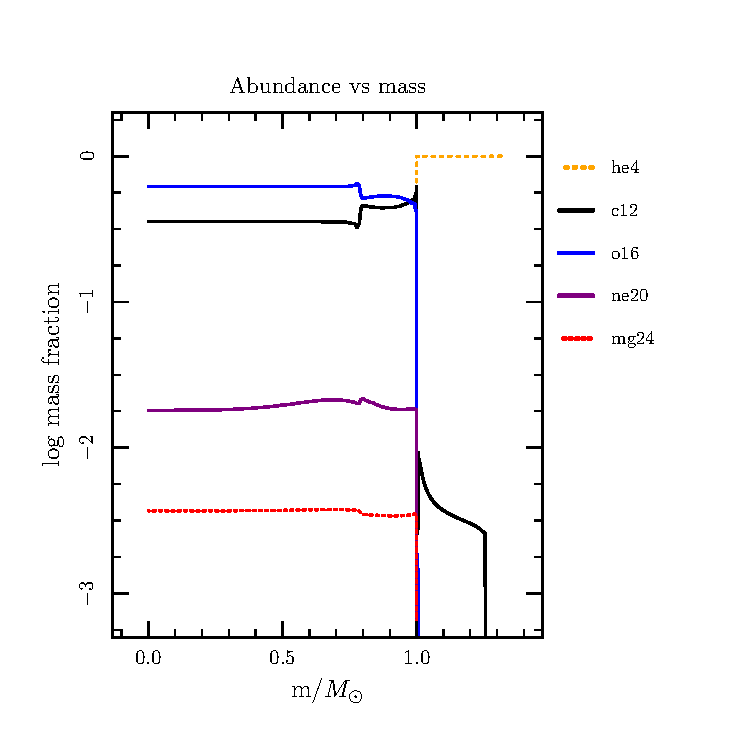
\includegraphics[width = 3.8in]{/Users/jaredbrooks/wd3/plots_out/Abundance_vs_mass_6.pdf}
	    \caption{Abundance profile showing}
	    \label{fig:1}
          \end{minipage}
          \hspace{0cm}
          \begin{minipage}[b]{0.5\linewidth}
            \centering
            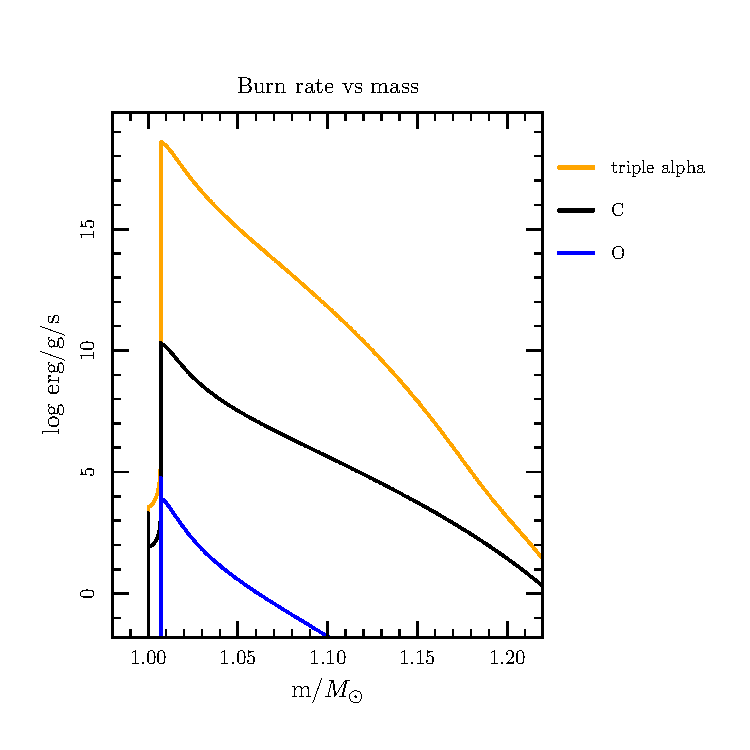
\includegraphics[width = 3.8in]{/Users/jaredbrooks/wd3/plots_out/Burnrate_vs_mass_6.pdf}
            \caption{Burning rate profile, peak triple-alpha burning at bottom of helium shell}
            \label{fig:4}
          \end{minipage}
	\end{figure}

        \pagebreak

        The helium luminosity (figure \ref{fig:5}) starts very low and increases gradually throughout the run until the sharp peak at 337 Myr reaches $10^{16}$.  The temperature-density profile from the end of the run (figure \ref{fig:7}) shows a temperature spike at the bottom of the helium shell.


        \begin{figure}[H]
          \begin{minipage}[b]{0.5\linewidth}
            \centering
            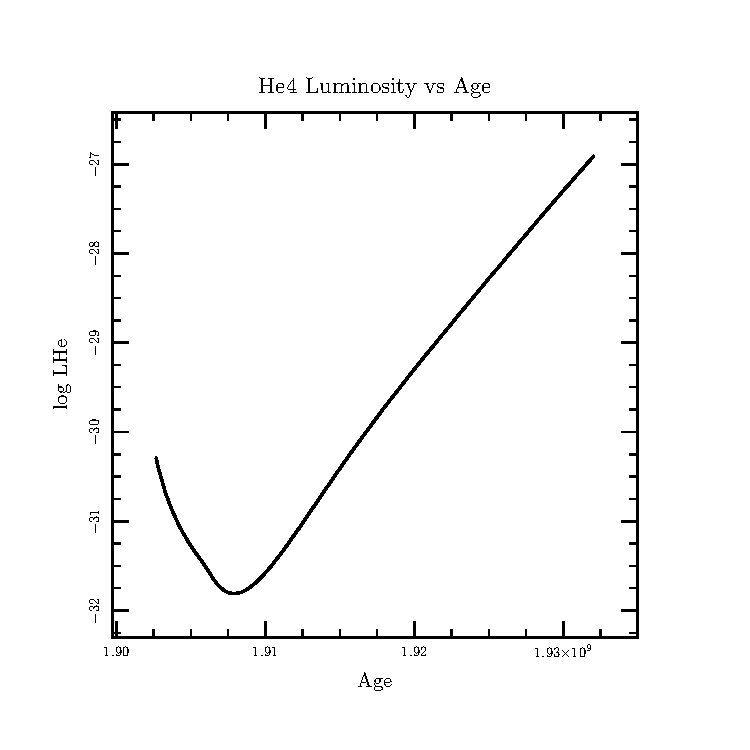
\includegraphics[width = 3.8in]{/Users/jaredbrooks/wd3/plots_out/He4_Luminosity_vs_Age.pdf}
            \caption{Helium Luminosity throughout the age of the model, gradual increase followed by a sharp peak at the end}
            \label{fig:5}
          \end{minipage}
          \hspace{0cm}
          \begin{minipage}[b]{0.5\linewidth}
            \centering
            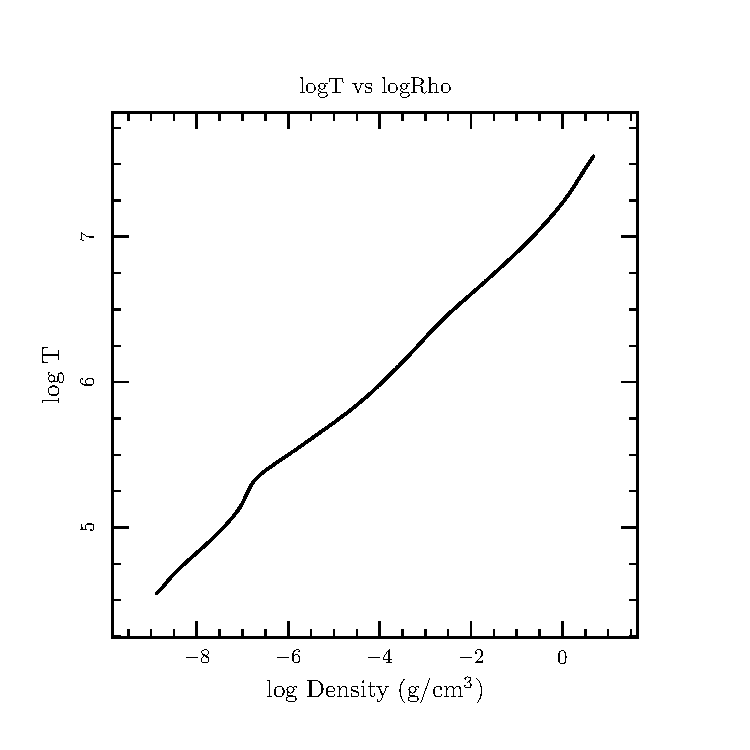
\includegraphics[width = 3.8in]{/Users/jaredbrooks/wd3/plots_out/Log_T_vs_logRho.pdf}
            \caption{Temperature-density profile from end of run, temperature spike at bottom of helium shell}
            \label{fig:7}
          \end{minipage}
        \end{figure}

        \pagebreak

        Before the peak in helium luminosity, however, overall luminosity (figure \ref{fig:2}) and effective temperature (figure \ref{fig:3}) are gradually inreasing due to heat released from the gravitational potential energy from the accreting helium.

        \begin{figure}[H]
          \begin{minipage}[b]{0.5\linewidth}
            \centering
            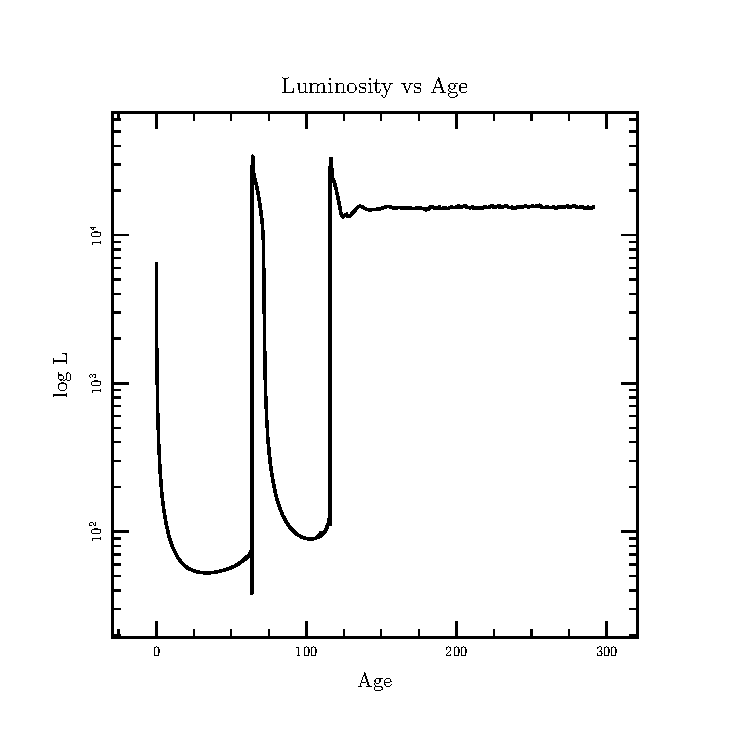
\includegraphics[width = 3.8in]{/Users/jaredbrooks/wd3/plots_out/Luminosity_vs_Age.pdf}
            \caption{\footnotesize Gradual luminosity increase from gravitation potential energy from accreting helium}
            \label{fig:2}
          \end{minipage}
          \hspace{0cm}
          \begin{minipage}[b]{0.5\linewidth}
            \centering
            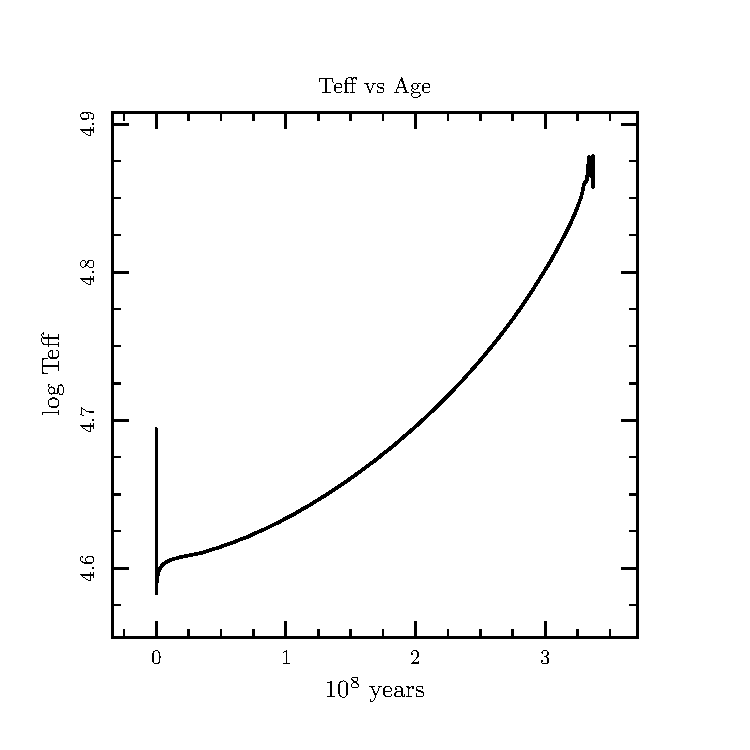
\includegraphics[width = 3.8in]{/Users/jaredbrooks/wd3/plots_out/Teff_vs_Age.pdf}
            \caption{\footnotesize Gradual effective temperature increase from gravitation potential energy from accreting helium}
            \label{fig:3}
          \end{minipage}
        \end{figure}

        \pagebreak

        This final plot (figure \ref{fig:6}) shows a few internal \texttt{MESA} variables, such as the size of the time-step, the number of zones, and the number of retries against the model number in order to give some understanding of how hard \texttt{MESA} is working throughout the run and where some areas of problems/interest might be.

        \begin{figure}[H]
                \centering
                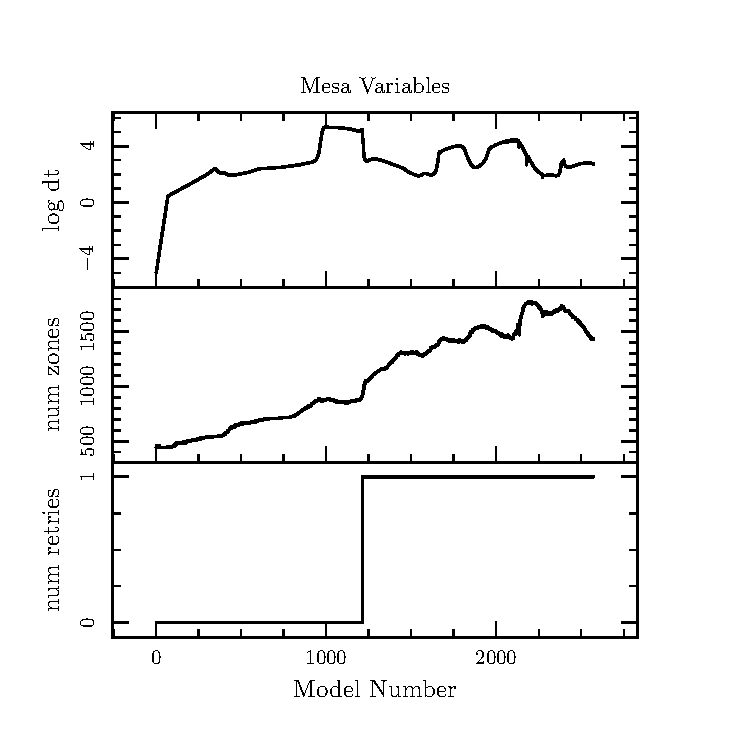
\includegraphics[width = 5in]{/Users/jaredbrooks/wd3/plots_out/Mesa_Variables.pdf}
                \caption{\texttt{MESA} variables plotted against model number show how hard \texttt{MESA} is working}
                \label{fig:6}
        \end{figure}

\end{document}
